\documentclass[14pt]{extbook}
\usepackage{multicol, enumerate, enumitem, hyperref, color, soul, setspace, parskip, fancyhdr} %General Packages
\usepackage{amssymb, amsthm, amsmath, bbm, latexsym, units, mathtools} %Math Packages
\everymath{\displaystyle} %All math in Display Style
% Packages with additional options
\usepackage[headsep=0.5cm,headheight=12pt, left=1 in,right= 1 in,top= 1 in,bottom= 1 in]{geometry}
\usepackage[usenames,dvipsnames]{xcolor}
\usepackage{dashrule}  % Package to use the command below to create lines between items
\newcommand{\litem}[1]{\item#1\hspace*{-1cm}\rule{\textwidth}{0.4pt}}
\pagestyle{fancy}
\lhead{Progress Quiz 4}
\chead{}
\rhead{Version C}
\lfoot{4378-7085}
\cfoot{}
\rfoot{Fall 2020}
\begin{document}

\begin{enumerate}
\litem{
Solve the quadratic equation below. Then, choose the intervals that the solutions belong to, with $x_1 \leq x_2$ (if they exist).\[ 17x^{2} +14 x -5 = 0 \]\begin{enumerate}[label=\Alph*.]
\item \( x_1 \in [-23.76, -23.39] \text{ and } x_2 \in [22.5, 23.25] \)
\item \( x_1 \in [-0.49, 0.53] \text{ and } x_2 \in [0.62, 1.57] \)
\item \( x_1 \in [-1.49, -0.4] \text{ and } x_2 \in [-0.4, 1] \)
\item \( x_1 \in [-18.75, -18.33] \text{ and } x_2 \in [4.31, 4.69] \)
\item \( \text{There are no Real solutions.} \)

\end{enumerate} }
\litem{
Graph the equation below.\[ f(x) = -(x-4)^2 + 19 \]\begin{enumerate}[label=\Alph*.]
\begin{multicols}{2}\item 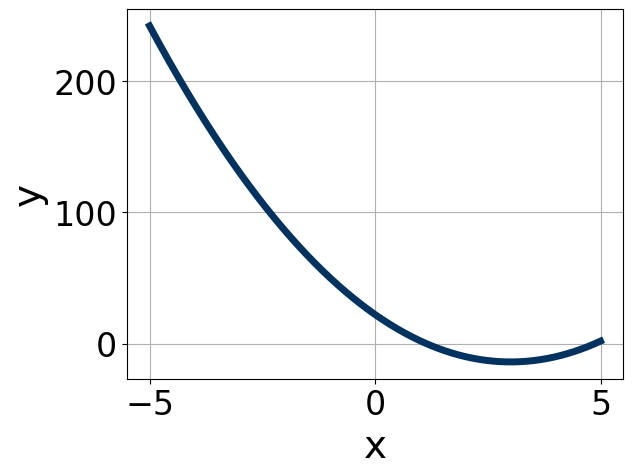
\includegraphics[width = 0.3\textwidth]{../Figures/quadraticEquationToGraphCopyAC.png}\item 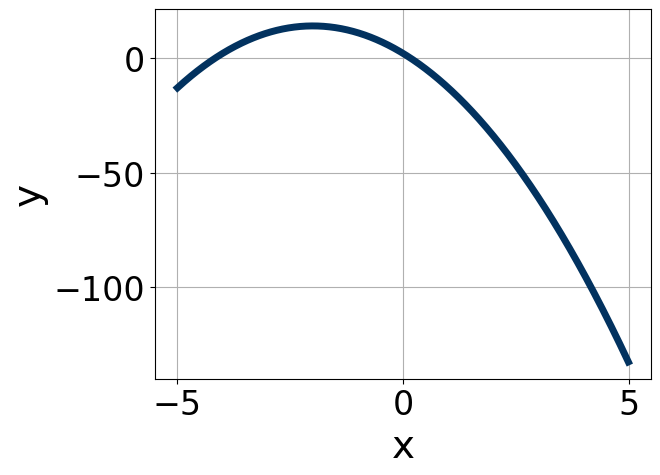
\includegraphics[width = 0.3\textwidth]{../Figures/quadraticEquationToGraphCopyBC.png}\item 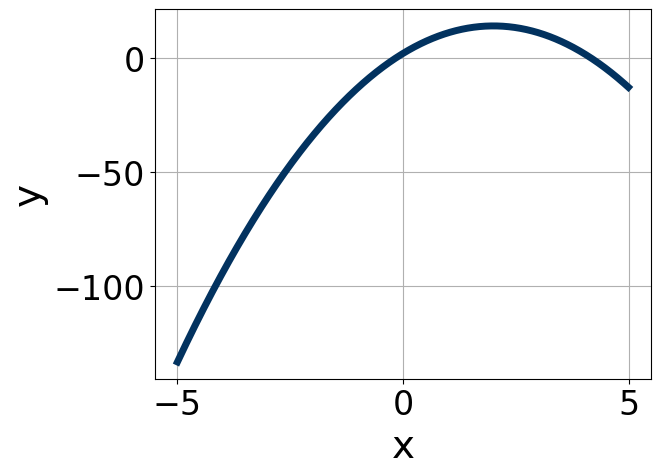
\includegraphics[width = 0.3\textwidth]{../Figures/quadraticEquationToGraphCopyCC.png}\item 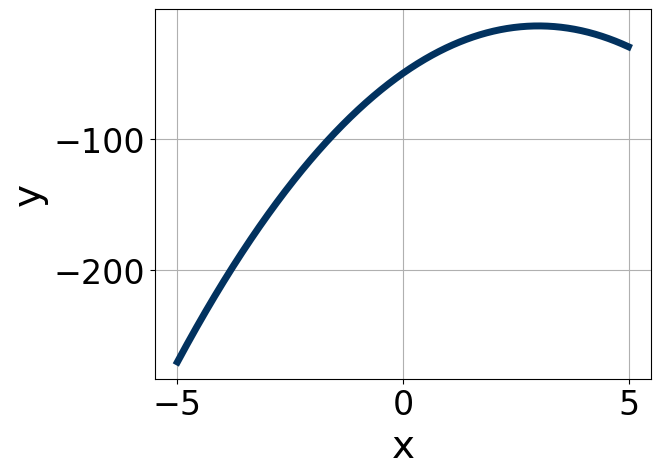
\includegraphics[width = 0.3\textwidth]{../Figures/quadraticEquationToGraphCopyDC.png}\end{multicols}\item None of the above.
\end{enumerate} }
\litem{
Factor the quadratic below. Then, choose the intervals that contain the constants in the form $(ax+b)(cx+d); b \leq d.$\[ 24x^{2} -2 x -15 \]\begin{enumerate}[label=\Alph*.]
\item \( a \in [11.7, 12.3], \hspace*{5mm} b \in [-7, 0], \hspace*{5mm} c \in [1.5, 3.9], \text{ and } \hspace*{5mm} d \in [3, 6] \)
\item \( a \in [4.8, 7.7], \hspace*{5mm} b \in [-7, 0], \hspace*{5mm} c \in [2.8, 5.1], \text{ and } \hspace*{5mm} d \in [3, 6] \)
\item \( a \in [2, 3.3], \hspace*{5mm} b \in [-7, 0], \hspace*{5mm} c \in [5.8, 8.8], \text{ and } \hspace*{5mm} d \in [3, 6] \)
\item \( a \in [-0.2, 2.2], \hspace*{5mm} b \in [-20, -18], \hspace*{5mm} c \in [-0.9, 1.7], \text{ and } \hspace*{5mm} d \in [15, 21] \)
\item \( \text{None of the above.} \)

\end{enumerate} }
\litem{
Factor the quadratic below. Then, choose the intervals that contain the constants in the form $(ax+b)(cx+d); b \leq d.$\[ 36x^{2} +11 x -12 \]\begin{enumerate}[label=\Alph*.]
\item \( a \in [-0.2, 1.7], \hspace*{5mm} b \in [-21, -15], \hspace*{5mm} c \in [-1.4, 2.8], \text{ and } \hspace*{5mm} d \in [26, 38] \)
\item \( a \in [1.5, 7.3], \hspace*{5mm} b \in [-6, 0], \hspace*{5mm} c \in [4.6, 10.4], \text{ and } \hspace*{5mm} d \in [2, 5] \)
\item \( a \in [8.4, 9.5], \hspace*{5mm} b \in [-6, 0], \hspace*{5mm} c \in [3.7, 4.3], \text{ and } \hspace*{5mm} d \in [2, 5] \)
\item \( a \in [26.9, 27.8], \hspace*{5mm} b \in [-6, 0], \hspace*{5mm} c \in [-1.4, 2.8], \text{ and } \hspace*{5mm} d \in [2, 5] \)
\item \( \text{None of the above.} \)

\end{enumerate} }
\litem{
Solve the quadratic equation below. Then, choose the intervals that the solutions belong to, with $x_1 \leq x_2$ (if they exist).\[ -14x^{2} +14 x + 2 = 0 \]\begin{enumerate}[label=\Alph*.]
\item \( x_1 \in [-2.2, -0.5] \text{ and } x_2 \in [-0.77, 0.44] \)
\item \( x_1 \in [-1.1, 0.5] \text{ and } x_2 \in [0.48, 1.55] \)
\item \( x_1 \in [-18.8, -16.5] \text{ and } x_2 \in [17.6, 19.49] \)
\item \( x_1 \in [-16.1, -15.2] \text{ and } x_2 \in [1.75, 1.89] \)
\item \( \text{There are no Real solutions.} \)

\end{enumerate} }
\litem{
Graph the equation below.\[ f(x) = -(x+4)^2 - 13 \]\begin{enumerate}[label=\Alph*.]
\begin{multicols}{2}\item 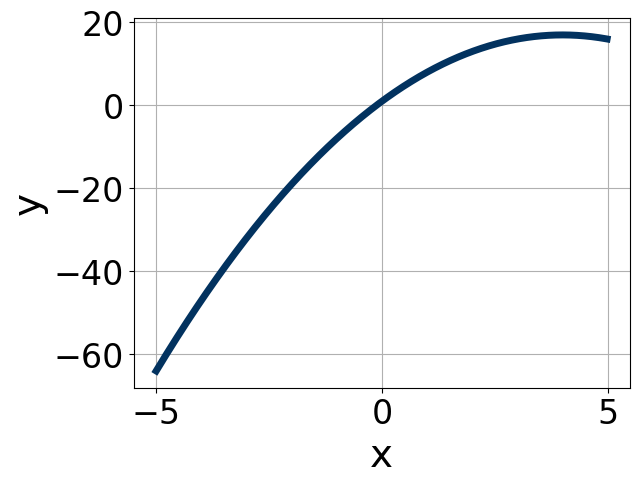
\includegraphics[width = 0.3\textwidth]{../Figures/quadraticEquationToGraphAC.png}\item 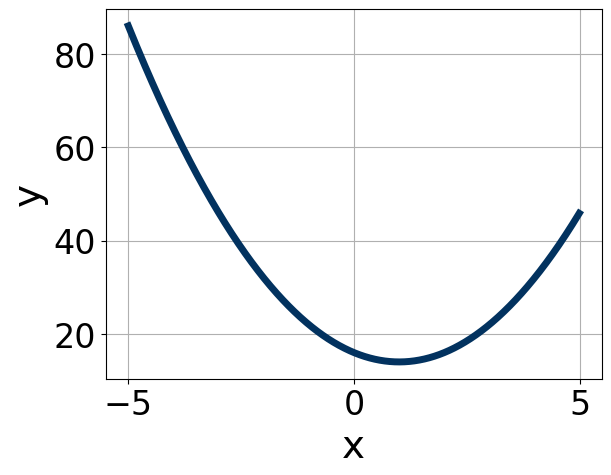
\includegraphics[width = 0.3\textwidth]{../Figures/quadraticEquationToGraphBC.png}\item 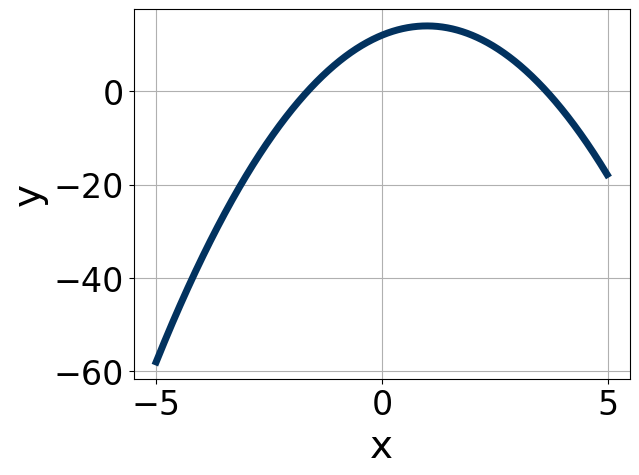
\includegraphics[width = 0.3\textwidth]{../Figures/quadraticEquationToGraphCC.png}\item 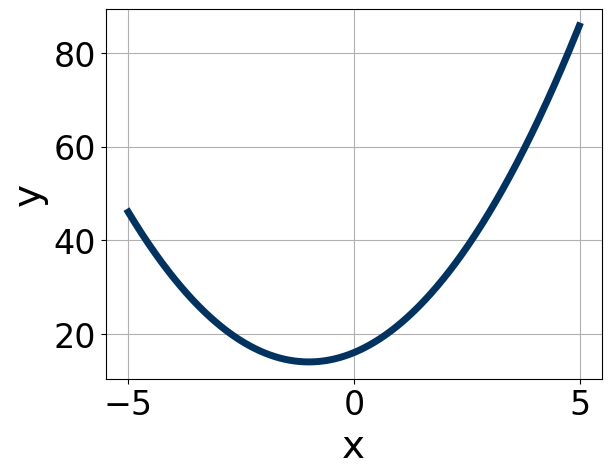
\includegraphics[width = 0.3\textwidth]{../Figures/quadraticEquationToGraphDC.png}\end{multicols}\item None of the above.
\end{enumerate} }
\litem{
Write the equation of the graph presented below in the form $f(x)=ax^2+bx+c$, assuming  $a=1$ or $a=-1$. Then, choose the intervals that $a, b,$ and $c$ belong to.
\begin{center}
    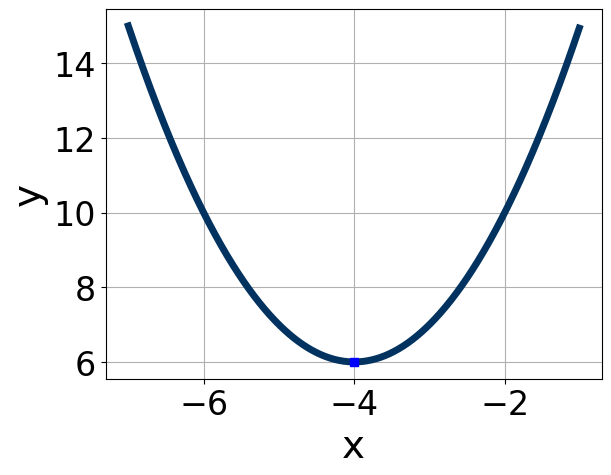
\includegraphics[width=0.5\textwidth]{../Figures/quadraticGraphToEquationC.png}
\end{center}
\begin{enumerate}[label=\Alph*.]
\item \( a \in [-1.8, -0.7], \hspace*{5mm} b \in [8, 10], \text{ and } \hspace*{5mm} c \in [-23, -21] \)
\item \( a \in [-0.5, 1.4], \hspace*{5mm} b \in [8, 10], \text{ and } \hspace*{5mm} c \in [9, 11] \)
\item \( a \in [-1.8, -0.7], \hspace*{5mm} b \in [-10, -6], \text{ and } \hspace*{5mm} c \in [-23, -21] \)
\item \( a \in [-1.8, -0.7], \hspace*{5mm} b \in [8, 10], \text{ and } \hspace*{5mm} c \in [-13, -8] \)
\item \( a \in [-0.5, 1.4], \hspace*{5mm} b \in [-10, -6], \text{ and } \hspace*{5mm} c \in [9, 11] \)

\end{enumerate} }
\litem{
Write the equation of the graph presented below in the form $f(x)=ax^2+bx+c$, assuming  $a=1$ or $a=-1$. Then, choose the intervals that $a, b,$ and $c$ belong to.
\begin{center}
    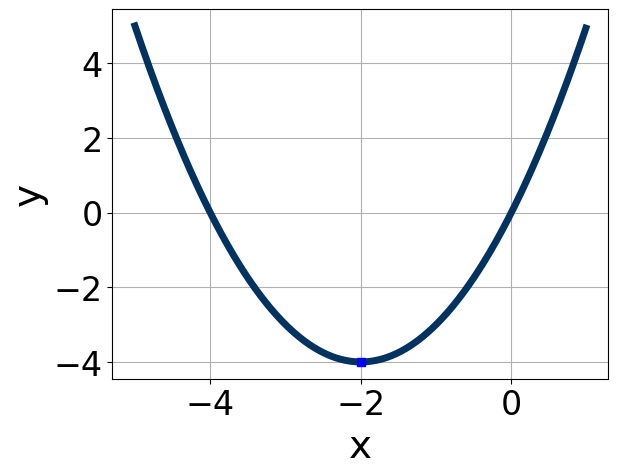
\includegraphics[width=0.5\textwidth]{../Figures/quadraticGraphToEquationCopyC.png}
\end{center}
\begin{enumerate}[label=\Alph*.]
\item \( a \in [1, 4], \hspace*{5mm} b \in [-9, -6], \text{ and } \hspace*{5mm} c \in [12, 15] \)
\item \( a \in [-3, 0], \hspace*{5mm} b \in [7, 11], \text{ and } \hspace*{5mm} c \in [-20, -18] \)
\item \( a \in [1, 4], \hspace*{5mm} b \in [-9, -6], \text{ and } \hspace*{5mm} c \in [18, 24] \)
\item \( a \in [1, 4], \hspace*{5mm} b \in [7, 11], \text{ and } \hspace*{5mm} c \in [12, 15] \)
\item \( a \in [-3, 0], \hspace*{5mm} b \in [-9, -6], \text{ and } \hspace*{5mm} c \in [-20, -18] \)

\end{enumerate} }
\litem{
Solve the quadratic equation below. Then, choose the intervals that the solutions $x_1$ and $x_2$ belong to, with $x_1 \leq x_2$.\[ 25x^{2} -10 x -24 = 0 \]\begin{enumerate}[label=\Alph*.]
\item \( x_1 \in [-1.37, -0.78] \text{ and } x_2 \in [1.2, 1.35] \)
\item \( x_1 \in [-4.46, -3.3] \text{ and } x_2 \in [0.1, 0.33] \)
\item \( x_1 \in [-20.65, -19.34] \text{ and } x_2 \in [29.82, 30.15] \)
\item \( x_1 \in [-1.95, -1.48] \text{ and } x_2 \in [0.52, 0.63] \)
\item \( x_1 \in [-0.53, -0.22] \text{ and } x_2 \in [2.3, 2.45] \)

\end{enumerate} }
\litem{
Solve the quadratic equation below. Then, choose the intervals that the solutions $x_1$ and $x_2$ belong to, with $x_1 \leq x_2$.\[ 6x^{2} -35 x + 36 = 0 \]\begin{enumerate}[label=\Alph*.]
\item \( x_1 \in [0.39, 0.49] \text{ and } x_2 \in [12.89, 13.77] \)
\item \( x_1 \in [7.79, 8.16] \text{ and } x_2 \in [26.95, 27.69] \)
\item \( x_1 \in [2.08, 2.71] \text{ and } x_2 \in [1.93, 3.23] \)
\item \( x_1 \in [1.2, 1.47] \text{ and } x_2 \in [4.04, 4.79] \)
\item \( x_1 \in [1.48, 1.61] \text{ and } x_2 \in [3.79, 4.38] \)

\end{enumerate} }
\end{enumerate}

\end{document}